\problemname{Digital Speedometer}
\par
A digital speedometer shows a vehicle's speed as integer miles per
hour.  There are occasions when the sensed speed varies between two
integer values, such as during cruise control.  Using a single
threshold to round between adjacent integers often makes the display
toggle rapidly between the two integers, which is distracting to the
driver.
\par
Your team must implement a smoothing technique for the display using 
separate rising and falling thresholds ($t_r$ and $t_f$, $t_f < t_r$, respectively).
% comment out the following line if Figure 1 is not used.
See Figure~1 for a graphical depiction of the Sample Input for use with
the following rules.
\begin{figure}[h]
	\begin{center}
		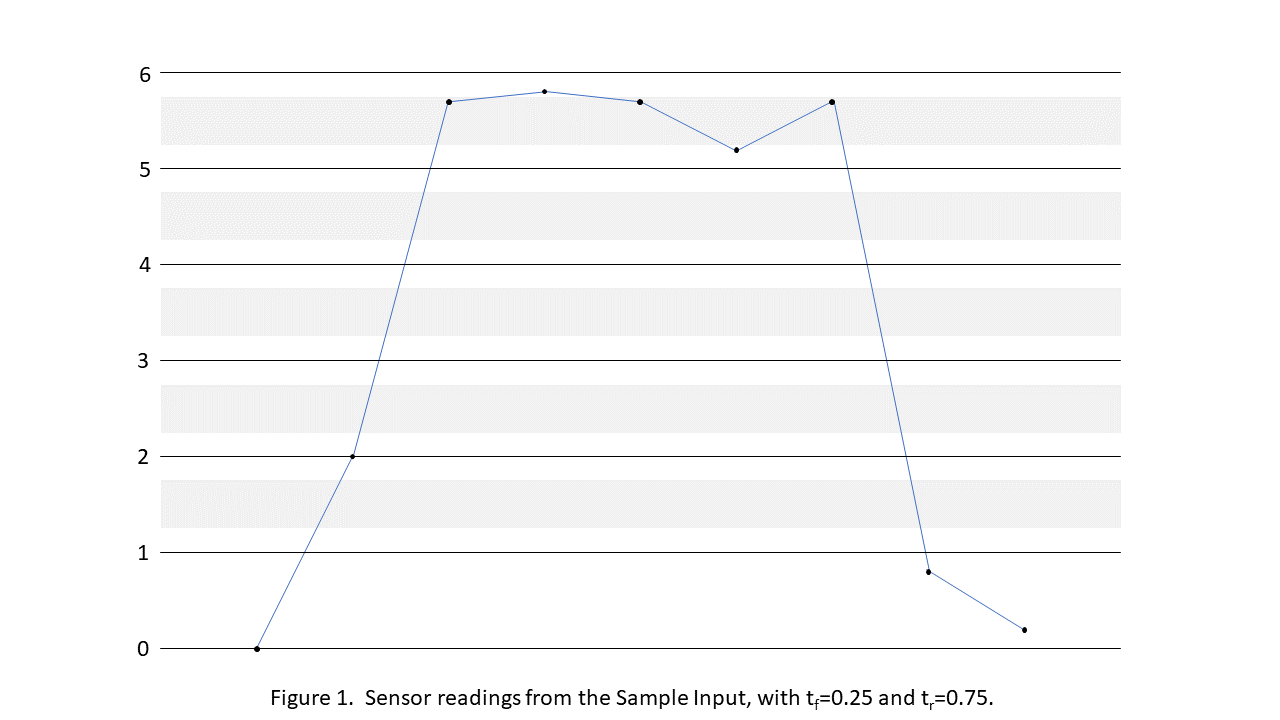
\includegraphics[width=0.9\textwidth]{speedometer-Figure-1.png}
	\end{center}
	\label{fig:sample}
\end{figure}
\par
%
Each sensed speed, $s$, falls between two adjacent integers $i$ and $j$,
$i \le s < j$, where $j = i + 1$.  When displaying the sensed speed $s$
as an integer:
\begin{itemize}
	\item When $s$ falls between $i$ and $i+t_f$, $s$ is displayed as $i$.
	\item When $s$ falls between $i+t_r$ and $j$, $s$ is displayed as $j$.
	\item When $s$ falls between $i+t_f$ and $i+t_r$, $s$ is displayed as $i$ if the most recent preceding value for $s$ outside of range $[i+t_f, i+t_r]$ is less than $i+t_r$, and $s$ is displayed as $j$ if the most recent preceding value for $s$ outside of range $[i+t_f, i+t_r]$ is greater than $i+t_r$.
	\item Any sensed speed, $0 < s < 1$, must display as $1$ because any non-zero speed,
	no matter how small, must display as non-zero to indicate that the vehicle is in motion.
\end{itemize}

\section*{Input}

The first line of input contains $t_f$, the falling threshold.  
The second line of input contains $t_r$, the rising threshold.
The speed sensor reports $s$ in increments of $0.1$ mph.  The thresholds
are always set halfway between speed increments.
All remaining lines until end-of-file are successive decimal speeds, $s$,
in miles per hour, one speed per line.  
The third line of input, which is the first measured speed, will always be $0$.
There are at most $1000$ observed speeds $s$ in input.
$$0 < t_f,t_r < 1; \ \ \ \ t_f < t_r; \ \ \ \ 0 \le s \le 120$$

\section*{Output}

\vskip -\parskip
Output is the list of speeds, one speed per line, smoothed to integer values appropriate to $t_f$ and $t_r$.

\section*{Sample Explanation}
\vspace{.5em}

\begin{tabular}{p{1cm} p{1cm} l}
	Input & Output & Explanation \\
	& & \\
	{\tt0.25} & & Value of $t_f$.\\
	{\tt 0.75}&&Value of $t_r$.\\
	{\tt 0}&{\tt 0}&Initial input.\\
	{\tt 2.0}&{\tt 2}&Input greater than $0$, below threshold of $2.25$.\\
	{\tt 5.7}&{\tt 5}&Input greater than $2.0$, in threshold range.\\
	{\tt 5.8}&{\tt 6}&Input greater than $2.0$, exceeds upper threshold
	of $5.75$.\\
	{\tt 5.7}&{\tt 6}&Input less than $5.8$, in threshold range.\\
	{\tt 5.2}&{\tt 5}&Input less than $5.8$, below threshold of $5.25$.\\
	{\tt 5.7}&{\tt 5}&Input greater than $5.2$, in threshold range.\\
	{\tt 0.8}&{\tt 1}&Input greater than $0$ and less than $1$.\\
	{\tt 0.2}&{\tt 1}&Input greater than $0$ and less than $1$.
\end{tabular}